% L9c lecture companion. Notebook hashes and coverage are recorded in README.md.
% Style files and Cornell seal are copied unchanged from the L7c deck (identical
% to L7a and L6c, which match the approved L6a deck). The logistic function and
% gradient descent figures are the light PDFs from ../figs, copied into assets/
% by `make figures`.
%
% Notation follows the lecture: augmented features \hat{x}_i, parameters
% theta = (w_1, ..., w_m, b), labels y in {-1, 1}, inverse temperature beta,
% cross-entropy loss J(theta), regularization parameter delta, and the
% augmented objective P_{mu,rho}(x) for simulated annealing. Greek vectors
% (theta) are set plain, as the notebook renders them and as the figures label
% them.
\documentclass[aspectratio=169,11pt]{beamer}
\usepackage{vnslides}
\renewcommand{\vnlecturecode}{L9c}
\newcommand{\lecturelink}{https://github.com/varnerlab/CHEME-5800-CourseRepository-Fall-2026/blob/main/weeks/week-09/L9c/CHEME-5800-L9c-Lecture-LogisticRegressionAndOptimization-Fall-2026.ipynb}
\newcommand{\examplelink}{https://github.com/varnerlab/CHEME-5800-CourseRepository-Fall-2026/blob/main/weeks/week-09/L9c/CHEME-5800-L9c-Example-LogisticRegression-GD-SA-Fall-2026.ipynb}
\newcommand{\advancedlink}{https://github.com/varnerlab/CHEME-5800-CourseRepository-Fall-2026/blob/main/weeks/week-09/L9c/CHEME-5800-L9c-Advanced-NonlinearOptimization-Fall-2026.ipynb}
\newcommand{\lablink}{https://github.com/varnerlab/CHEME-5800-CourseRepository-Fall-2026/blob/main/weeks/week-09/L9d/CHEME-5800-L9d-Lab-LogisticRegression-Banknotes-Fall-2026.ipynb}
\newcommand{\lecturesource}[1]{\note{[Sources]\par
  \href{\lecturelink}{L9c lecture: Logistic Regression and Numerical Optimization.}\par
  #1\par[/Sources]}}
\newcommand{\xh}{\hat{\mathbf x}}
\newcommand{\Xh}{\hat{\mathbf X}}
\newcommand{\thh}{\hat{\theta}}
\newcommand{\Pt}{P_{\theta}}

\title{\texorpdfstring{{\vnheavy L9c}}{L9c}: Logistic Regression and Numerical Optimization}
\subtitle{\texorpdfstring{The logistic model, gradient descent, and simulated annealing\\[3pt]CHEME 5800 Cornell University}{The logistic model, gradient descent, and simulated annealing; CHEME 5800 Cornell University}}
\author{Copyright Jeffrey Varner 2026. All Rights Reserved}

\begin{document}
\special{pdf:minorversion 7}
\vntitlepage

\begin{frame}{Objectives for Today}
  How can a linear classifier report how confident it is, and how do we
  estimate its parameters when no formula gives them directly?

  \vspace{0.4em}
  {\large\textbf{\ink{Today's concepts}}}
  \vspace{0.2em}
  \begin{itemize}\setlength{\itemsep}{0.4em}
    \item \hilite{Derive the logistic regression model for binary classification}:
      derive the logistic function from the Boltzmann distribution and use its
      probabilities to assign class labels.
    \item \hilite{Estimate logistic regression parameters with gradient descent}:
      minimize the cross-entropy loss with its gradient, and add a penalty on
      the size of the parameters.
    \item \hilite{Solve constrained problems with simulated annealing}: fold the
      constraints into the objective with penalty and barrier terms, and choose
      the temperature schedule.
  \end{itemize}
  \slidenote{Lecture:}{\href{\lecturelink}{Logistic Regression and Numerical Optimization}}
  \lecturesource{Introduction and three Learning Objectives.}
\end{frame}

\begin{frame}{Lecture and Example}
  \textbf{\ink{Lecture:}}
  \href{\lecturelink}{Logistic Regression and Numerical Optimization}

  In this lecture, we derive logistic regression, estimate its parameters with
  gradient descent, and solve constrained problems with simulated annealing.

  \vspace{1.1em}
  \textbf{\ink{Example:}}
  \href{\examplelink}{Fit a Logistic Regression Classifier}

  In this example, we fit a logistic regression model to two overlapping
  clusters with gradient descent and with simulated annealing, which never
  computes a gradient, and compare the two answers.

  \vspace{0.8em}
  Unlike the Perceptron, logistic regression predicts a class label and the
  probability behind it.
  \lecturesource{Introduction and Examples.}
\end{frame}

\begin{frame}{From the Sign Function to a Probability}
  The Perceptron labels an example by the sign of the score $\xh^\top\theta$.
  \hilite{Logistic regression} replaces the sign with a probability that rises
  smoothly with the score.

  \vspace{0.2em}
  \centering
  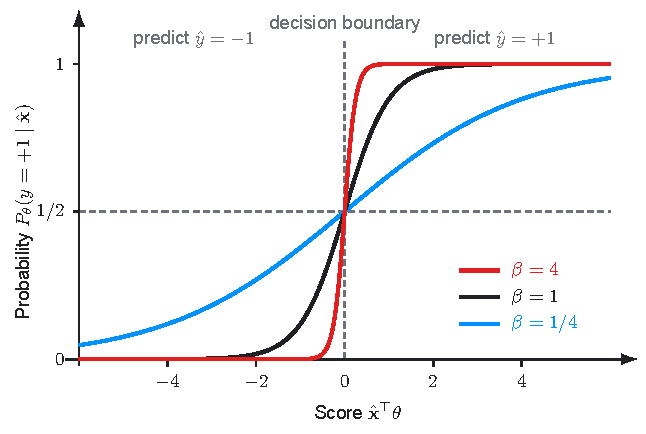
\includegraphics[width=\textwidth,height=0.47\paperheight,keepaspectratio]{assets/Fig-Logistic-Function.pdf}

  \vspace{0.2em}
  \raggedright
  Each curve is the probability of $y=+1$ for one inverse temperature $\beta$.
  Every curve crosses $1/2$ at the decision boundary; a larger $\beta$ makes the
  rise sharper.
  \lecturesource{Logistic Regression: opening paragraph, figure, and caption.
    Figure: ../figs/Fig-Logistic-Function (TikZ, October 9, 2026).}
\end{frame}

\begin{frame}{Labels as States in a Boltzmann Distribution}
  We treat the labels $y\in\{-1,1\}$ as \hilite{states} of a Boltzmann
  distribution conditioned on $\xh$, where lower-energy states are more
  probable. With energy $E(y,\xh)$ and inverse temperature $\beta=1/T>0$:
  \[
    P(y\mid\xh)=\frac{\exp\bigl(-\beta E(y,\xh)\bigr)}
      {\underbrace{\textstyle\sum_{y'\in\{-1,1\}}\exp\bigl(-\beta E(y',\xh)\bigr)}_{Z(\xh)}}
  \]
  The partition function $Z(\xh)$ normalizes the probabilities. For the
  energy, we use a linear model:
  \[
    E(y,\xh)=-\,y\bigl(\xh^\top\theta\bigr).
  \]
  A large positive score $\xh^\top\theta$ gives $y=+1$ the lower energy, so it
  is more probable; a very negative score favors $y=-1$.
  \lecturesource{Logistic Regression: Derivation, Boltzmann distribution, partition function, and energy function.}
\end{frame}

\begin{frame}{Deriving the Logistic Function}
  Substitute the energy and let $z=\beta\,\xh^\top\theta$:
  \[
    \begin{aligned}
      \Pt(y\mid\xh)
      &=\frac{\exp(yz)}{\exp(z)+\exp(-z)}
      =\frac{1}{\exp\bigl((1-y)z\bigr)+\exp\bigl(-(1+y)z\bigr)}.
    \end{aligned}
  \]
  Evaluating the two cases:
  \[
    \Pt(y=+1\mid\xh)=\frac{1}{1+\exp\bigl(-2\beta\,\xh^\top\theta\bigr)},
    \qquad
    \Pt(y=-1\mid\xh)=\frac{1}{1+\exp\bigl(2\beta\,\xh^\top\theta\bigr)}.
  \]
  Together, these give the \hilite{logistic function}
  $\sigma(z)=1/\bigl(1+e^{-z}\bigr)$:
  \[
    \boxed{\Pt(y\mid\xh)=\frac{1}{1+\exp\bigl(-2\beta y\,\xh^\top\theta\bigr)}
      =\sigma\bigl(2\beta y\,\xh^\top\theta\bigr)}
  \]
  The logistic function maps any real input into $(0,1)$, and
  $\sigma(-z)=1-\sigma(z)$, so the two label probabilities sum to one.
  \lecturesource{Logistic Regression: Derivation, algebra, Cases callout, and the closing paragraph.}
\end{frame}

\begin{frame}{The Inverse Temperature $\beta$}
  The inverse temperature $\beta>0$ sets how \hilite{confident} the model is
  in its decisions:

  \vspace{0.5em}
  \begin{itemize}\setlength{\itemsep}{0.8em}
    \item \hilite{Large $\beta$ (cold system)}: small energy differences give
      large probability differences. As $\beta\to\infty$, the logistic function
      becomes the Perceptron's hard threshold.
    \item \hilite{Small $\beta$ (hot system)}: the states become nearly equally
      probable. As $\beta\to0$, each label's probability approaches $1/2$.
  \end{itemize}

  \vspace{0.7em}
  In practice, $\beta$ appears only in the product $\beta\,\theta$, so we fix
  $\beta$ and learn $\theta$. Setting $\beta=1/2$ gives the common form
  $\Pt(y\mid\xh)=\sigma\bigl(y\,\xh^\top\theta\bigr)$.
  \lecturesource{Understanding the Inverse Temperature: Physical intuition callout and In practice paragraph.}
\end{frame}

\begin{frame}{From Probabilities to Class Labels}
  To classify an example, we predict the more probable label:
  \[
    \hat y=
    \begin{cases}
      +1 & \text{if } \Pt(y=+1\mid\xh)\ge1/2,\\
      -1 & \text{otherwise}.
    \end{cases}
  \]
  Because $\sigma(z)\ge1/2$ exactly when $z\ge0$, this is the Perceptron's
  rule $\hat y=\texttt{sign}(\xh^\top\theta)$, with the same decision boundary.

  \vspace{0.6em}
  \hilite{Choosing a threshold.} We can instead predict $\hat y=+1$ when the
  probability is at least some threshold $t\in(0,1)$. Lowering $t$ labels
  more examples positive, so the recall and the number of false positives can
  only rise or stay the same.

  \vspace{0.5em}
  When a missed positive is costly, as in disease screening, a threshold
  below $1/2$ may be better.
  \lecturesource{From Probabilities to Class Labels: decision rule and Choosing a threshold.}
\end{frame}

\begin{frame}{The Cross-Entropy Loss}
  For a dataset $\mathcal D=\{(\mathbf x_i,y_i)\mid i=1,\ldots,n\}$ of
  independent examples, we choose the parameters that make the observed
  labels most likely:
  \[
    \mathcal L(\theta)=\prod_{i=1}^{n}\Pt(y_i\mid\xh_i)
    \quad\Longrightarrow\quad
    \log\mathcal L(\theta)=-\sum_{i=1}^{n}\log\Bigl(1+\exp\bigl(-2\beta y_i\,\xh_i^\top\theta\bigr)\Bigr).
  \]
  Taking the log turns the product into a sum. Minimizing the
  negative log-likelihood, the \hilite{cross-entropy loss}, gives the estimate:
  \[
    \boxed{J(\theta)=\sum_{i=1}^{n}\log\Bigl(1+\exp\bigl(-2\beta y_i\,\xh_i^\top\theta\bigr)\Bigr)},
    \qquad
    \thh=\arg\min_{\theta}J(\theta).
  \]
  Unlike least squares, $\nabla J(\theta)=\mathbf 0$ has no closed-form
  solution, so we minimize $J(\theta)$ \hilite{numerically}.
  \lecturesource{Parameter Estimation: Learning from Data: likelihood, log-likelihood, boxed cross-entropy loss, and the closing sentence.}
\end{frame}

\begin{frame}{Gradient Descent and Local Minima}
  The gradient points in the direction of steepest increase, so gradient
  descent steps \hilite{opposite the gradient}.

  \vspace{0.2em}
  \centering
  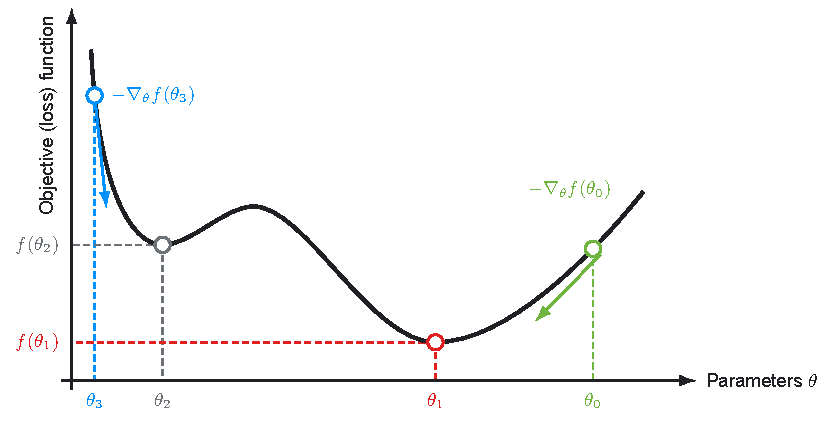
\includegraphics[width=\textwidth,height=0.5\paperheight,keepaspectratio]{assets/Fig-GD-Schematic.pdf}

  \vspace{0.2em}
  \raggedright
  Started at $\theta_0$, it reaches the lowest point $\theta_1$; started at
  $\theta_3$, it stops at $\theta_2$, a \hilite{local minimum}.
  \lecturesource{Gradient Descent: figure, caption, and the Gradient? callout.
    Figure: ../figs/Fig-GD-Schematic (TikZ, October 9, 2026).}
\end{frame}

\begin{frame}{Gradient of the Cross-Entropy Loss}
  Let $u_i=2\beta y_i\,\xh_i^\top\theta$, so term $i$ of the loss is
  $\log\bigl(1+e^{-u_i}\bigr)$. By the chain rule:
  \[
    \nabla_{\theta}\log\bigl(1+e^{-u_i}\bigr)
    =\left(\frac{-e^{-u_i}}{1+e^{-u_i}}\right)\nabla_{\theta}u_i
    =-\bigl(1-\sigma(u_i)\bigr)\,2\beta y_i\,\xh_i.
  \]
  Summing over the training examples:
  \[
    \boxed{\nabla J(\theta)=-2\beta\sum_{i=1}^{n}\bigl(1-\sigma(u_i)\bigr)\,y_i\,\xh_i}
  \]
  The factor $1-\sigma(u_i)$ is the probability the model gives to the
  \hilite{wrong label} for example $i$, so each step adds every $y_i\,\xh_i$,
  weighted by this probability.

  \vspace{0.5em}
  The Perceptron update uses only the mistakes, each with full weight; here,
  confidently correct examples contribute almost nothing.
  \lecturesource{Gradient Descent: Gradient of the cross-entropy loss callout and the comparison with the Perceptron update.}
\end{frame}

\begin{frame}{Gradient Descent Algorithm}
  \textbf{Initialize}: Choose $\theta^{(0)}$ (random or zeros), a
  learning rate $\alpha(k)>0$, a tolerance $\epsilon>0$, and $\texttt{maxiter}$.
  Set $\texttt{converged}\gets\texttt{false}$ and $k\gets0$.

  \vspace{0.4em}
  While not $\texttt{converged}$ \textbf{do}:
  \begin{enumerate}\setlength{\itemsep}{0.2em}
    \item Compute the direction $\mathbf d=-\nabla J\bigl(\theta^{(k)}\bigr)$.
    \item Update $\theta^{(k+1)}=\theta^{(k)}+\alpha(k)\,\mathbf d$.
    \item Check the stopping criterion:
      \begin{itemize}\setlength{\itemsep}{0.1em}
        \item If $\|\theta^{(k+1)}-\theta^{(k)}\|_2\le\epsilon$, \textbf{then} set
          $\texttt{converged}\gets\texttt{true}$ and return $\theta^{(k+1)}$.
        \item If $k+1\ge\texttt{maxiter}$, \textbf{then} return $\theta^{(k+1)}$
          and warn that it did not converge.
      \end{itemize}
    \item Increment $k\gets k+1$, and update $\alpha(k)$, if applicable.
  \end{enumerate}

  \vspace{0.3em}
  Too large a \hilite{learning rate} may overshoot the minimum; too small a
  rate converges slowly. We can also stop when
  $\|\nabla J(\theta^{(k)})\|_2\le\epsilon$.
  \lecturesource{Gradient Descent Algorithm: pseudocode and the two components. Preserve the Initialize/While/numbered-step format.}
\end{frame}

\begin{frame}{Convexity of the Loss}
  A function $f$ is \hilite{convex} if, for any inputs $\mathbf a,\mathbf b$
  and any weight $t\in[0,1]$:
  \[
    f\bigl(t\,\mathbf a+(1-t)\,\mathbf b\bigr)\le t\,f(\mathbf a)+(1-t)\,f(\mathbf b).
  \]
  The line segment connecting any two points on the graph lies on or above the
  graph. For example, $x^2$ and $e^x$ are convex, while $-x^2$ is not.

  \vspace{0.6em}
  A convex function has no local minimum like $\theta_2$ in the figure:
  \hilite{any local minimum is a global minimum}.

  \vspace{0.6em}
  Each term of the cross-entropy loss is a convex function of $u_i$, which is
  linear in $\theta$, so $J(\theta)$ is convex.
  \lecturesource{How Good Is Gradient Descent?: Convexity callout and the convexity of J.}
\end{frame}

\begin{frame}{How Good Is Gradient Descent?}
  \begin{itemize}\setlength{\itemsep}{0.6em}
    \item \hilite{A safe learning rate}: the gradient is Lipschitz, so with
      $\alpha\le1/L$, every step lowers the loss unless the gradient is zero:
      \[
        \|\nabla J(\mathbf a)-\nabla J(\mathbf b)\|_2\le L\,\|\mathbf a-\mathbf b\|_2,
        \qquad L=\beta^2\|\Xh\|_2^2,
      \]
      where $\|\Xh\|_2$ is the largest singular value of the data matrix.
    \item \hilite{Slowing down over time}: when the loss has a minimizer, the
      gap to the optimal loss after $k$ steps shrinks like $1/k$. We sprint
      at first, then settle into a steady jog.
    \item \hilite{When there is no minimum}: on linearly separable data,
      scaling up a separating $\theta$ lowers every term of the loss, so
      $\theta$ keeps growing. Regularization fixes this.
  \end{itemize}
  \slidenote{Advanced:}{\href{\advancedlink}{Momentum methods, Newton's method, and constrained gradient descent}}
  \lecturesource{How Good Is Gradient Descent?: the three bullets and the pointer to the advanced notebook.}
\end{frame}

\begin{frame}{Regularization: Preventing Overfitting}
  To keep the model from following the training data too closely, we add a
  ridge penalty on the size of the parameters:
  \[
    \boxed{J_\delta(\theta)=J(\theta)+\frac{\delta}{2}\,\|\theta\|_2^2},
    \qquad
    \nabla J_\delta(\theta)=\nabla J(\theta)+\delta\,\theta,
  \]
  where $\delta\ge0$ is the \hilite{regularization parameter}. We minimize
  $J_\delta$ with gradient descent.

  \vspace{0.4em}
  With $\delta>0$, the loss is \hilite{strongly convex}: it has exactly one
  minimizer, even for separable data, and each step with
  $\alpha\le1/(L+\delta)$ shrinks the gap to the minimum loss by at least a
  constant fraction.

  \vspace{0.4em}
  \begin{itemize}\setlength{\itemsep}{0.3em}
    \item \hilite{Scale the features} to comparable magnitudes, so the penalty
      treats the parameters fairly.
    \item \hilite{Choose $\delta$ by cross-validation}, as we did for ridge
      regression.
  \end{itemize}
  \lecturesource{Regularization: Preventing Overfitting: boxed loss, gradient, strong convexity, and the In practice callout.}
\end{frame}

\begin{frame}{Constrained Problems}
  Many engineering problems restrict their decision variables, for example,
  to fractions that must be nonnegative and sum to one. We minimize a
  nonlinear objective $f(x)$ subject to $m$ inequality and $p$ equality
  constraints:
  \[
    \min_{x\in\mathbb R^n}\;f(x)
    \quad\text{s.t.}\quad
    \begin{cases}
      g_i(x)\le0, & i=1,\ldots,m,\\
      h_j(x)=0, & j=1,\ldots,p.
    \end{cases}
  \]

  \vspace{0.4em}
  Logistic regression has no constraints on $\theta$. Simulated annealing,
  like gradient descent, works on an unconstrained objective, so we fold the
  constraints into it.
  \slidenote{Advanced:}{\href{\advancedlink}{The Karush--Kuhn--Tucker conditions and a gradient method for this problem}}
  \lecturesource{Constrained Problems and Simulated Annealing: problem statement and the advanced-notebook pointer; Penalty and Barrier Terms: opening sentence.}
\end{frame}

\begin{frame}{Penalty and Barrier Terms}
  A \hilite{penalty} grows with the size of a constraint violation. A
  \hilite{barrier} grows without bound as $x$ approaches the edge of the
  region where the inequality constraints hold:
  \[
    P_{\mu,\rho}(x)=f(x)
    \;-\;\underbrace{\mu\sum_{i=1}^{m}\ln\bigl(-g_i(x)\bigr)}_{\text{barrier term}}
    \;+\;\underbrace{\frac{1}{2\rho}\sum_{j=1}^{p}\bigl[h_j(x)\bigr]^2}_{\text{penalty term}},
    \qquad\mu>0,\;\rho>0.
  \]
  The logarithmic barrier keeps the solution strictly inside the region. We
  decrease both parameters over the iterations:
  \begin{itemize}\setlength{\itemsep}{0.5em}
    \item \hilite{Barrier weight}: as $\mu\to0$, the barrier fades inside the
      region, so the solution can approach its edge, where the optimum often
      lies.
    \item \hilite{Penalty weight}: as $\rho\to0$, the coefficient $1/\rho$
      grows, enforcing the equality constraints more strictly.
  \end{itemize}
  \lecturesource{Penalty and Barrier Terms: Penalty and barrier methods callout, augmented objective, and Parameters callout.}
\end{frame}

\begin{frame}{Simulated Annealing}
  \hilite{Simulated annealing} (Kirkpatrick, Gelatt, and Vecchi, 1983) is a
  derivative-free method inspired by annealing in metallurgy: heating a metal
  and cooling it slowly so its atoms settle into a low-energy arrangement.

  \vspace{0.6em}
  It accepts both improving and non-improving moves, controlled by a
  \hilite{temperature} $T$. A move that raises the objective by $\Delta P>0$
  is accepted with probability:
  \[
    p_{\text{accept}}=\exp\bigl(-\Delta P/T\bigr),
  \]
  the Boltzmann factor from our derivation with $\beta=1/T$.

  \vspace{0.4em}
  \begin{itemize}\setlength{\itemsep}{0.4em}
    \item At a \hilite{high temperature}, uphill moves are often accepted.
    \item As $T$ \hilite{decreases}, they become rare.
  \end{itemize}
  \lecturesource{Simulated Annealing: opening paragraph and Why does this work?}
\end{frame}

\begin{frame}{Escaping a Local Minimum}
  Started at $\theta_3$, simulated annealing moves downhill to $\theta_2$,
  where gradient descent stops.

  \vspace{0.2em}
  \centering
  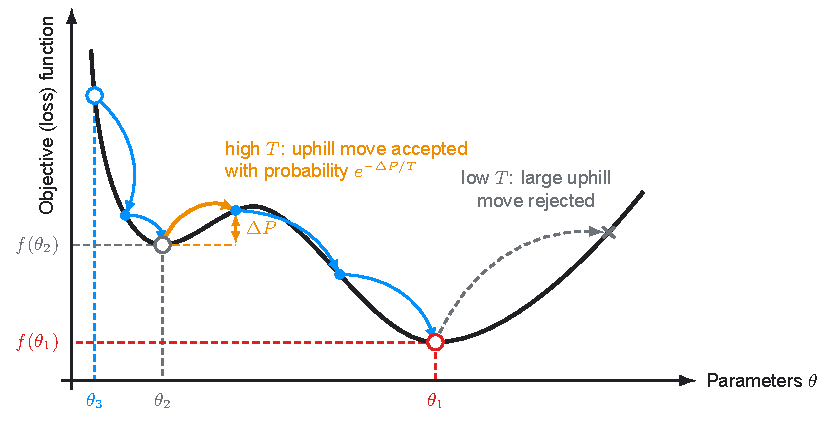
\includegraphics[width=\textwidth,height=0.5\paperheight,keepaspectratio]{assets/Fig-SA-Schematic.pdf}

  \vspace{0.2em}
  \raggedright
  At a \hilite{high temperature}, it accepts an uphill move, then moves downhill
  to $\theta_1$; at a \hilite{low temperature}, it rejects a large uphill move.
  \lecturesource{Simulated Annealing: figure and its caption paragraph.
    Figure: ../figs/Fig-SA-Schematic (TikZ, October 19, 2026).}
\end{frame}

\begin{frame}{Simulated Annealing: Setup}
  \textbf{Initialize}: Given:
  \begin{itemize}\setlength{\itemsep}{0.35em}
    \item an initial solution $x_0$ with $g_i(x_0)<0$ for all $i$,
    \item penalty parameters $\mu,\rho>0$ with update factors
      $\tau_\mu,\tau_\rho\in(0,1)$,
    \item an initial temperature $T\gets T_\circ$ and a minimum temperature
      $T_{\min}$, with $T_\circ>T_{\min}>0$,
    \item a cooling rate $\alpha\in(0,1)$, a step size $\eta>0$, and the number
      of iterations $K$ per temperature.
  \end{itemize}

  \vspace{0.5em}
  Set $\texttt{converged}\gets\texttt{false}$, the best solution
  $x^\star\gets x_0$, and the current solution $x_c\gets x_0$.

  \vspace{0.6em}
  The equality constraints enter only through the penalty term, so at the end
  we check how close each $h_j(x^\star)$ is to zero.
  \lecturesource{Simulated Annealing: Initialize, and the sentence after the pseudocode on the equality constraints.}
\end{frame}

\begin{frame}{Simulated Annealing: The Loop}
  While not $\texttt{converged}$ \textbf{do}:
  \begin{enumerate}\setlength{\itemsep}{0.2em}
    \item For $k=1$ to $K$ \textbf{do}:
      \begin{itemize}\setlength{\itemsep}{0.1em}
        \item Generate a candidate $x'\gets x_c+\eta\cdot\texttt{randn}(\texttt{size}(x_c))$.
        \item If $g_i(x')\ge0$ for any $i$, \textbf{then} reject it; the barrier is
          undefined there.
        \item Compute $\Delta P\gets P_{\mu,\rho}(x')-P_{\mu,\rho}(x_c)$.
          If $\Delta P<0$, accept: $x_c\gets x'$. Otherwise, draw
          $u\sim\texttt{Uniform}(0,1)$ and accept if $u\le\exp(-\Delta P/T)$.
        \item If $P_{\mu,\rho}(x_c)<P_{\mu,\rho}(x^\star)$, \textbf{then} set
          $x^\star\gets x_c$, with both values at the current $\mu,\rho$.
      \end{itemize}
    \item Update the penalty parameters: $\mu\gets\tau_\mu\,\mu$ and
      $\rho\gets\tau_\rho\,\rho$.
    \item If $T\le T_{\min}$, \textbf{then} set
      $\texttt{converged}\gets\texttt{true}$ and return $x^\star$.
      Otherwise, cool: $T\gets\alpha\,T$.
  \end{enumerate}

  \vspace{0.3em}
  Here, $\texttt{randn}$ draws independent normal random numbers with mean
  zero and variance one.
  \lecturesource{Simulated Annealing: While loop. Preserve the While/numbered-step/nested-conditional format.}
\end{frame}

\begin{frame}{Selecting $T_\circ$ and $K$}
  Simulated annealing is a \hilite{heuristic}: it does not guarantee the global
  minimum, and its result depends on the temperature schedule.

  \vspace{0.5em}
  \textbf{\ink{Sample-and-set rule for $T_\circ$.}}
  From $x_0$, generate $M=100$ candidates, discard any that violate an
  inequality constraint, and average the uphill changes $\Delta P_j>0$ to get
  $\overline{\Delta P}_+$. Choose the probability $p_\circ\in(0.6,0.9)$ of
  accepting an average uphill move at the start, and set:
  \[
    T_\circ=-\frac{\overline{\Delta P}_+}{\ln p_\circ},
    \qquad\text{so that}\qquad
    \exp\bigl(-\overline{\Delta P}_+/T_\circ\bigr)=p_\circ.
  \]

  \vspace{0.2em}
  \textbf{\ink{Heuristic for $K$.}}
  Start with $K=\lceil c\,n\rceil$, where $n$ is the number of decision
  variables and $c\in[10,50]$. After each temperature, compute the acceptance
  rate $\hat p$: if $\hat p>0.8$, set $K\gets\lceil0.75K\rceil$; if
  $\hat p<0.2$, set $K\gets\lceil1.5K\rceil$.
  \lecturesource{Selecting T and K: Sample-and-set approach and Heuristic for choosing K.}
\end{frame}

\begin{frame}{Example: Fit a Logistic Regression Classifier}
  In this example, we fit one logistic regression model to two overlapping
  clusters of points with both methods.

  \vspace{0.6em}
  \begin{enumerate}\setlength{\itemsep}{0.6em}
    \item Fit the model with gradient descent, with the learning rate
      $\alpha=1/L$ computed from the training data, and watch the loss fall.
    \item Draw the probability contours and the decision boundary, and classify
      the testing points at several thresholds.
    \item Fit the same model with simulated annealing, choosing $T_\circ$ with
      the sample-and-set rule, and compare the two answers.
  \end{enumerate}

  \vspace{0.6em}
  Simulated annealing reaches nearly the same parameters without the
  gradient, at the cost of many more loss evaluations.
  \slidenote{Example:}{\href{\examplelink}{Fit a logistic regression classifier with gradient descent and simulated annealing}}
  \lecturesource{Selecting T and K: example callout.
    Companion example: Tasks 1--3 and the third key takeaway.}
\end{frame}

\begin{frame}{Lab: Logistic Regression for Banknotes}
  In the \href{\lablink}{lab}, we train a logistic regression classifier with
  gradient descent on the banknotes from the Perceptron example:

  \vspace{0.6em}
  \begin{itemize}\setlength{\itemsep}{0.6em}
    \item complete the training loop for the \hilite{regularized
      cross-entropy loss},
    \item evaluate the classifier with a \hilite{confusion matrix} and compare
      it with the classical and pocket Perceptron on the same banknotes, and
    \item use the \hilite{predicted probabilities} to decide which banknotes a
      person should check by hand.
  \end{itemize}

  \vspace{0.7em}
  The probability tells us which banknotes the classifier is unsure about.
  \slidenote{Lab:}{\href{\lablink}{Logistic regression with gradient descent on the banknotes}}
  \lecturesource{Lab section. Lab notebook: introduction and Learning Objectives.}
\end{frame}

\begin{frame}{Summary}
  We derived logistic regression from the Boltzmann distribution, fit it with
  gradient descent, and solved constrained problems with simulated annealing.

  \vspace{0.4em}
  {\large\textbf{\ink{Key takeaways}}}
  \vspace{0.3em}
  \begin{itemize}\setlength{\itemsep}{0.4em}
    \item \textbf{\ink{The logistic regression model.}} We treated the labels as
      Boltzmann states and derived the logistic function; predicting the more
      probable label recovers the Perceptron's decision boundary.
    \item \textbf{\ink{Parameter estimation with gradient descent.}} We minimized
      the cross-entropy loss, weighting each example by its wrong-label
      probability; a ridge penalty gives a unique minimizer.
    \item \textbf{\ink{Constrained problems and simulated annealing.}} We folded
      constraints in with penalty and barrier terms; accepting some uphill
      moves lets the search escape local minima.
  \end{itemize}

  \vspace{0.4em}
  The example and lab apply these ideas to synthetic clusters and to the
  banknotes.
  \lecturesource{Summary: three key takeaways and concluding sentence.}
\end{frame}

\end{document}
